% This text is proprietary.
% It's a part of presentation made by myself.
% It may not used commercial.
% The noncommercial use such as private and study is free
% Dec 2007
% Author: Sascha Frank 
% University Freiburg 
% www.informatik.uni-freiburg.de/~frank/
%
% 

\documentclass[12pt,a4paper,utf8x]{beamer}
\setbeamertemplate{navigation symbols}{}

\usepackage [frenchb]{babel}
\usepackage{color}
% Pour pouvoir utiliser 
\usepackage{ucs}
\usepackage[utf8x]{inputenc}

\usepackage{amsmath}

\usetheme{Malmoe}


\AtBeginSection[]
{
\begin{frame}{Plan}
\tableofcontents[currentsection]
 \end{frame}
}




\addtobeamertemplate{footline}{\hfill\insertframenumber/\inserttotalframenumber} 

\beamersetuncovermixins{\opaqueness<1>{25}}{\opaqueness<2->{15}}
\begin{document}
\title{Wikitty Publication}  
\author{Manoël Fortun}

\begin{frame}
\titlepage
\end{frame}

\begin{frame}\tableofcontents	
\end{frame} 


\section{Code Lutin}

\begin{frame}\frametitle{Code Lutin} 
\begin{itemize}
\item SSLL
\item Créée en 2002
\item Technologies JAVA
\item Des solutions Libres
\item Valeurs du Libre appliquées à l'entreprise
\end{itemize}
\end{frame}



\section{Wikitty} 
\subsection*{Présentation} 
\begin{frame}\frametitle{Présentation} 
\begin{itemize}
\item Base de données orientées colonnes
\item Clé $\to$ Valeur 
\item Super Objet : Wikitty
\item Getter/Setter avec le nom des champs
\item Mécanisme d'extension
\end{itemize}
\end{frame}


\subsection*{Des extentions} 
\begin{frame}\frametitle{Des extentions} 
\begin{itemize}
\item Définitions des champs : nomExtension.nomChamp
\item Génération depuis un modèle
\item Héritage d'extension
\item Objets Entités
\item concentration sur le métier
\end{itemize}
\end{frame}

\begin{frame}\frametitle{Des extentions} 
\begin{figure}
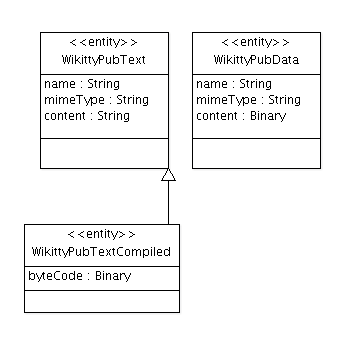
\includegraphics[scale=0.5]{../image/wikittypubuml.png} 
\caption{Exemple de diagramme}
\end{figure}
\end{frame}


\subsection*{Wikitty Service}
\begin{frame} \frametitle{Wikitty Service et Proxy} 
\begin{itemize}
\item Restauration 
\item Sauvegarde
\item Recherche
\item Configuré par fichier de propriétés
\item Stockage masqué
\end{itemize}
\end{frame}


\section{Le scripting}
\subsection*{Qu'es ce c'est ?}
\begin{frame}\frametitle{Qu'es ce c'est ?}

Ca permet d'interpréter et d'éxécuter un langage de script avec un autre langage.


\vspace{5mm}
Par exemple, interpréter et éxécuter du \emph{javascript} par du \emph{java}.
\end{frame}
\subsection*{Bindings}
\begin{frame}\frametitle{Bindings}
Très important, ça permet d'insérer des éléments du langage qui interprète, dans le script.\\
\vspace{5mm}
Par exemple dans le cas java, javascript ça permet dans d'insérer dans le javascript:
\begin{itemize}
\item Instanciation d'objet java
\item Invocation de méthode sur les objets
\end{itemize}
\end{frame}


\section{Wikitty Publication} 
\subsection*{Motivations}
\begin{frame}\frametitle{Motivations}

Des applications web que l'on peut modifier et utiliser dans un navigateur.\pause


\begin{figure}\pause
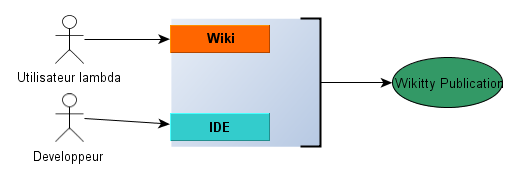
\includegraphics[scale=0.5]{../image/wpwhy.png} 
\caption{Motivations}
\end{figure}

\end{frame}

\subsection*{Comment ?}
\begin{frame} 
\begin{itemize}
\item Utilise le concept du scripting
\item Script stocké sous forme de Wikitty
\item WikittyPubText pour les script
\item WikittyPubData pour les données binaires
\item Moteur d'évaluation en Bindings
\end{itemize}

\end{frame}


\subsection*{Nouveau type de wikitty service}
\begin{frame}\frametitle{Nouveau type de wikitty service}
\begin{itemize}
\item wikitty service sur système de fichier
\item wikitty service sur jar
\item wikitty service fallback\pause
\end{itemize}\pause
\begin{figure}
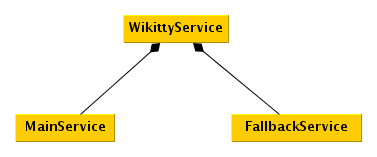
\includegraphics[scale=0.5]{../image/multicontext.png} 
\caption{Service avec fallback}
\end{figure}
\end{frame}



\subsection*{Synchronisation entre service}
\begin{frame}\frametitle{Synchronisation entre service}
\begin{itemize}
\item Transférer des wikitty d'un service à un autre
\item Basé sur l'extension WikittyLabel
\item Mise à jour
\item "Suppression"
\item "Déplacement" de wikitty
\end{itemize}
\pause
Exemple de label :
\verb!org.nuiton.wikitty!
\end{frame}

\begin{frame}
Exemple de synchronisation:
\begin{itemize}
\item cajo://localhost:1111\#com
\item cajo://wwikitty.nuiton.org:2222\#org
\end{itemize}
\vspace{5mm}
Les wikitty sous le label \verb!com! contenu sur le premier service vont
être envoyé sur le second service sous le label org.
\vspace{5mm}
Le label \verb!com.nuiton.wikitty! deviendra \verb!org.nuiton.wikitty! sur 
le second service.
\end{frame}

\subsection*{Externalisation}
\begin{frame}\frametitle{Externalisation}
\begin{itemize}
\item "Fixer" les wikitty
\item Compiler les scripts
\item Création d'un jar
\item WikittyPubTextCompiled
\end{itemize}
\end{frame}

\subsection*{Migration vers struts}
\begin{frame}\frametitle{Migration vers struts}
\begin{itemize}
\item Migration depuis une application en jsp "classic/simple"
\item Mécanisme de login/logout
\item action struts/interceptor
\item support struts pour les sessions etc
\end{itemize}
\end{frame}




\subsection*{Moteur d'évaluation}
\begin{frame}\frametitle{Moteur d'évaluation}

Moteur d'évaluation dans un navigateur à l'adresse:\\
\verb!/[contextData]/[contextApps]/[action]/[mandatory]!

\begin{itemize}
\item mandatory pour retrouver le wikitty correspondant
\item action, c'est le nom de l'action
\item contextApps, pour ne pas se tromper de wikitty.
\item contextData, pour trouver le bon wikitty service
\end{itemize}



\end{frame}
\begin{frame}\frametitle{Moteur d'évaluation}
Les actions :
\begin{itemize}
\item eval, évaluation du code
\item raw, rendu en fonction du type mime
\item edit, édition/création de wikitty
\item view, moteur de recherche, affichage wikitty
\end{itemize}



\end{frame}


\begin{frame}\frametitle{Moteur d'évaluation}

Comment ça marche contextData:

\begin{figure}
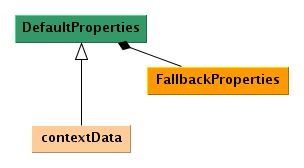
\includegraphics[scale=0.5]{../image/propertiescontext.png} 
\caption{Surcharge des propriétés}
\end{figure}

\end{frame}

\begin{frame}\frametitle{Moteur d'évaluation}
Le mime type des WikittyPub détermine le traitement effectué.
\begin{itemize}
\item text/javascript, passera par l'évaluateur de javascript
\item image/png, renvoyé tel quel en mettant le bon type mime dans la réponse 
pour interprétation du navigateur
\item text/html.javascript, passera par un décorateur pour transformer le contenu
en text/javascript pour interprétation
\item text/java, sera compilé pour évaluation
\end{itemize}
\end{frame}

\begin{frame}\frametitle{Moteur d'évaluation}

Exemple:
\verb!codelutin/chorem/eval/Menu! 

On va "évaluer" le wikittyPub qui possède le nom "Menu" avec un label qui
commence par "chorem" et qui se trouve dans le service correspondant à Code Lutin.
Le rendu sera déterminé par le mime Type du wikittyPub correspondant.
\end{frame}





\section*{Wikitty Struts} 
\begin{frame}\frametitle{Wikitty Struts}
Création d'une Tag lib struts pour une intégration facilité de wikitty dans des 
formulaire.
Deux possibilités d'utilisation
\begin{itemize}
\item Formulaire d'édition de wikitty, avec action pré-construite 
\item Intégration des champs de wikitty dans un formulaire, avec choix de la forme
de l'affichage en fonction du tag utilisé.
\end{itemize}

\end{frame}


\section{Plugin Maven}
\subsection*{Un plugin?!}
\begin{frame}\frametitle{Un plugin?!}
\begin{itemize}
\item Motivation: Plus simple pour l'utilisateur
\item Clés en mains
\item Intègre de façon ciblée les fonctionnalités (externalize-synchronize)
\end{itemize}
%pom exemple
%liste des goals
\end{frame}	

\subsection*{Les goals}
\begin{frame}\frametitle{Les goals}
\begin{itemize}
\item wp:init
\item wp:run
\item wp:deploy
\item wp:update
\item wp:jar
\item wp:jar-deploy
\end{itemize}

\end{frame}	

\section{Conclusion}
\begin{frame}\frametitle{Conclusion}

\end{frame}	


\end{document}
